\begin{figure}[htbp]
    \caption{PIT and QQ-plot}
    \label{fig:fig_pit_qqplot}
    \centering

	\subfloat[PIT]{
	    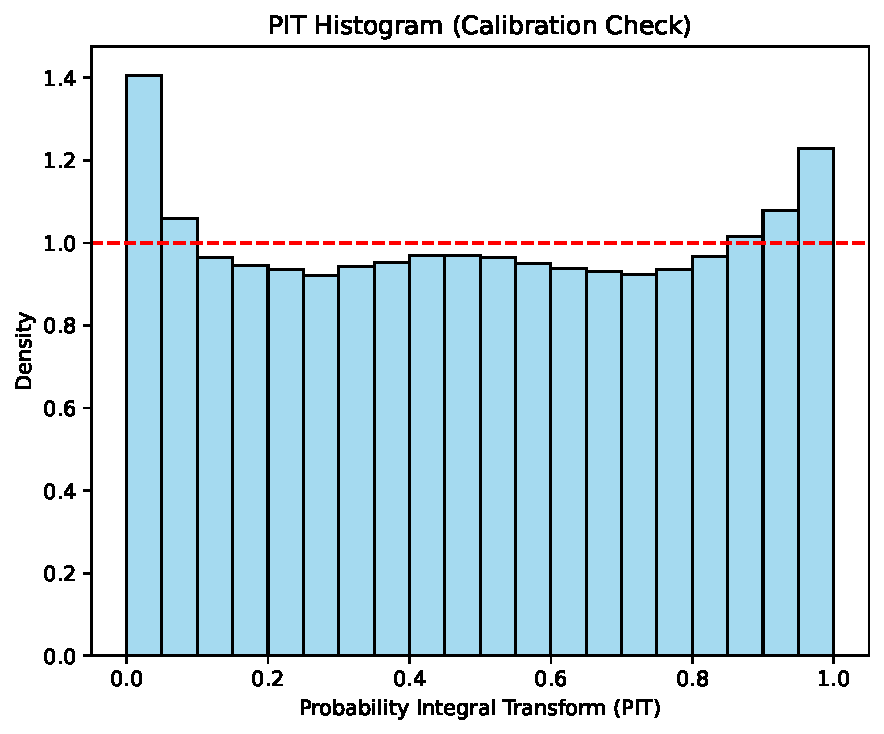
\includegraphics[width=0.48\textwidth]{fig/pit_histogram.pdf}
	 }
	\subfloat[QQ-plot]{
	    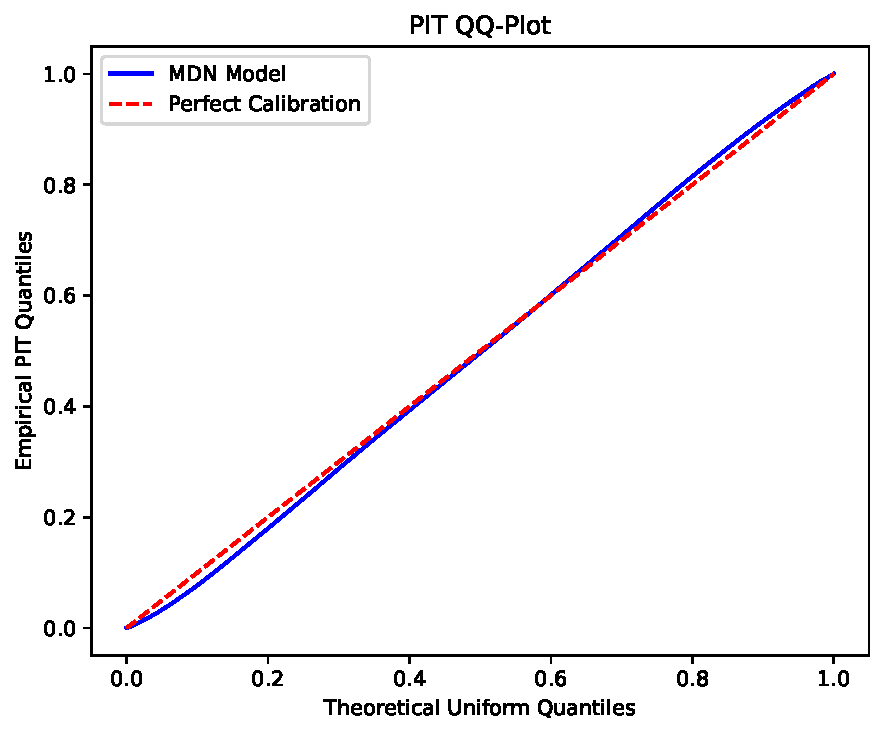
\includegraphics[width=0.48\textwidth]{fig/pit_qq_plot.pdf}
	 }
    % \vspace{0.2cm}
 %    \begin{minipage}{0.95\textwidth} 
	% {\footnotesize Now see how we can have two panels! \ldots
	% \par
	% }
	% \end{minipage}
\end{figure}




% \begin{figure}[htbp]
%     \centering
    
%     % 左图
%     \begin{minipage}[b]{0.48\textwidth}
%         \centering
%         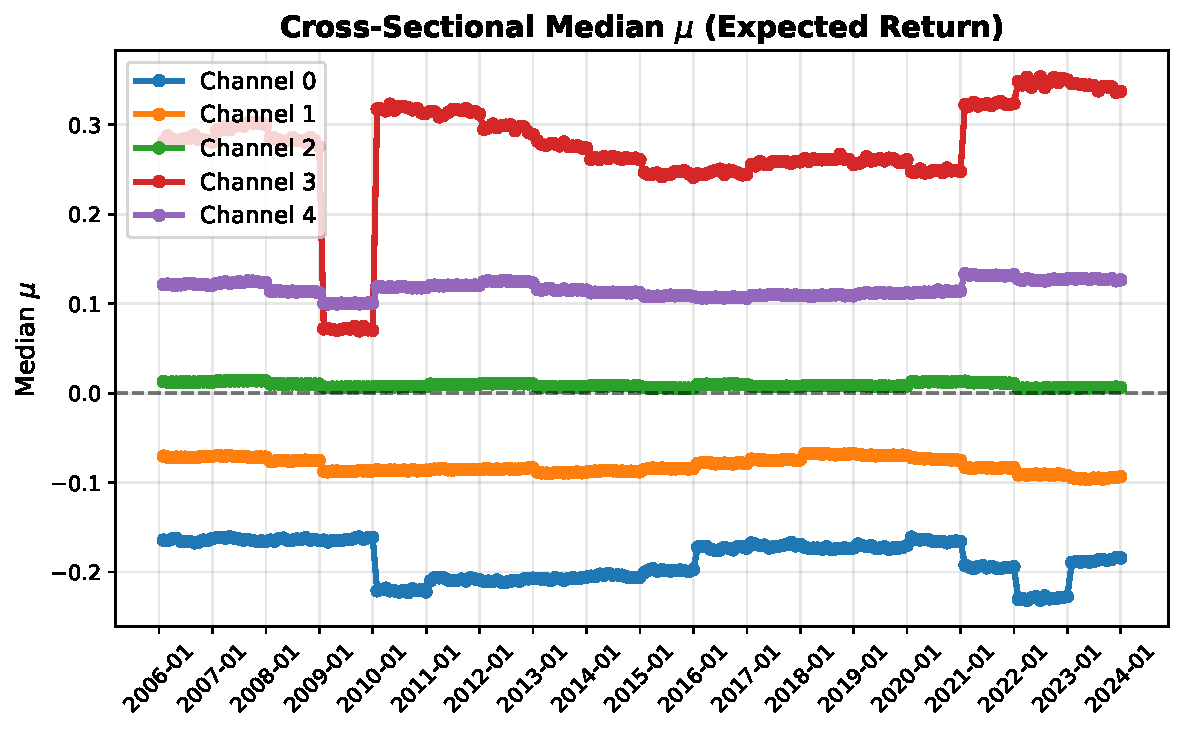
\includegraphics[width=\textwidth]{fig/regime_mu_all.pdf}
%         \vspace{0.1cm}
%         \centerline{(a) Title of Left Figure}
%     \end{minipage}
%     \hfill
%     % 右图
%     \begin{minipage}[b]{0.48\textwidth}
%         \centering
%         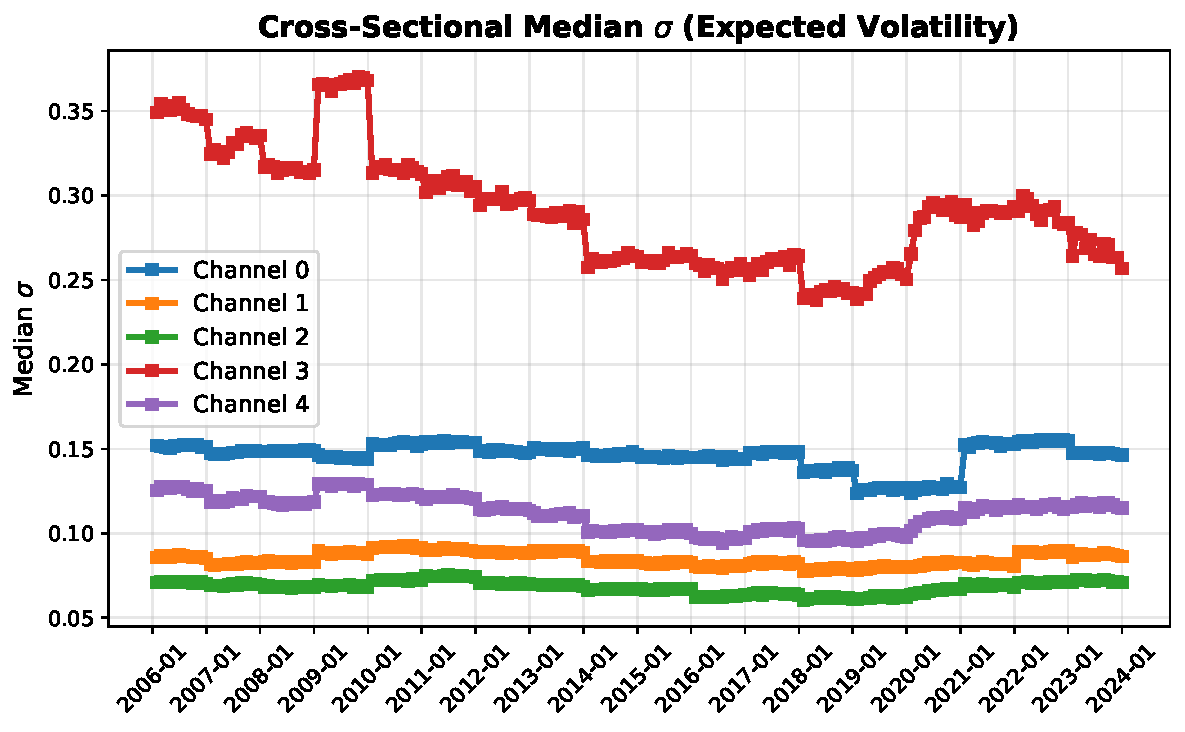
\includegraphics[width=\textwidth]{fig/regime_sigma_all.pdf}
%         \vspace{0.1cm}
%         \centerline{(b) Title of Right Figure}
%     \end{minipage}
    
%     \caption{This is the main caption for both figures.}
%     \label{fig:fig_pit_qqplot}
% \end{figure}